%TODO: more didactics (team work, ..)
%TODO: learning outcomes
%TODO: move recapitulation into front and make it according the learning outcomes
%TODO: some time for (TISS) feedback

% Make nice A4 pages for print:
%\usepackage{pgfpages}
%\pgfpagesuselayout{resize to}[a4paper,border shrink=5mm,landscape]

\beamertemplatenavigationsymbolsempty

\setbeamertemplate{bibliography item}[text]

\usepackage[type={CC},modifier={by-sa},version={4.0}]{doclicense}

\usepackage[utf8]{inputenc}
\usepackage{hyperref}
\usepackage{breakurl}
\usepackage{graphicx}
\usepackage{pgfplots}
\usepackage{pgf}
\usepackage{tikz}
\usetikzlibrary{positioning}
\usetikzlibrary{arrows}
\usetikzlibrary{decorations.markings}
\usetikzlibrary{calc}
\usetikzlibrary{matrix}
\usetikzlibrary{shapes}
\usetikzlibrary{decorations.pathmorphing}
\usetikzlibrary{fit}
\usetikzlibrary{backgrounds}
\usetikzlibrary{plotmarks}
\usepackage{stmaryrd}
\usepackage{listings}
\usepackage{pdflscape}
\usepackage{perpage}
\usepackage{appendixnumberbeamer}

%\usepackage[thmmarks,amsmath,amsthm]{ntheorem} % already included in beamer
\usepackage{thm-restate}

\usepackage[sort&compress,numbers]{natbib}  % to be have \citet, \citeauthor, \citeyear

\MakePerPage{footnote}

\tikzstyle{o}=[r,ppBlue]
\tikzstyle{r}=[thick,rectangle,align=center]
\tikzstyle{t}=[r,ppTrans] %,font=\bfseries]
\tikzstyle{dd}=[densely dashed]
\tikzstyle{n}=[r,ppBlue]
\tikzstyle{p}=[r,ppRed]
\tikzstyle{ppRed}  =[draw=red,  fill=  red!20]
\tikzstyle{ppBlue} =[draw=blue, fill= blue!20]
\tikzstyle{ppGreen}=[draw=green,fill=green!20]
\tikzstyle{ppTrans}=[draw=none, fill=none]

\usetheme{Warsaw}

\useoutertheme[subsection=true]{smoothbars}
%\useoutertheme[subsection=false]{miniframes}

\definecolor{bblue}{HTML}{D7DF01}	% yellow-ish actually, for better black/white printing
\definecolor{rred}{HTML}{C0504D}
\definecolor{ggreen}{HTML}{9BBB59}
\definecolor{ppurple}{HTML}{9F4C7C}
\definecolor{lightgray}{rgb}{0.3,0.3,0.3}
\definecolor{lightergray}{rgb}{0.9,0.9,0.9}
\definecolor{UniBlue}{RGB}{83,121,170}

\DeclareTextFontCommand\textintro{\normalfont\bfseries\itshape} % nice!
\newcommand{\intro}[2][]
{%
	\textintro{#2}%
}
\newcommand{\empha}[2][]
{%
	\emph{#2}%
}

%\theoremstyle{plain}
\newcounter{reqcounter}
\newtheorem{requirement}[reqcounter]{Requirement}

%setbeamercolor{structure}{fg=violet}

\makeatletter
\def\th@task{%
    \normalfont % body font
    \setbeamercolor{block title example}{bg=orange,fg=white}
    \setbeamercolor{block body example}{bg=orange!20,fg=black}
    \def\inserttheoremblockenv{exampleblock}
  }
\makeatother

\theoremstyle{task}
\newtheorem{task}{Task}

\newenvironment{assignment}%
{%\setbeamercolor{background canvas}{bg=violet}%
%\setbeamercolor{structure}{fg=cyan!90!black}%
 \setbeamercolor{frametitle}{bg=orange,fg=white}
\begin{frame}}%
{\end{frame}}%

\AtBeginSection[]{
  \begin{frame}
  \vfill
  \centering
  \begin{beamercolorbox}[sep=8pt,center,shadow=true,rounded=true]{title}
    \usebeamerfont{title}\insertsectionhead\par%
  \end{beamercolorbox}
  \tableofcontents
  \vfill
  \end{frame}
}




\pgfplotsset{compat=1.14}
\author{Markus Raab}


\date{19.6.2019}

\begin{document}

\renewcommand{\enquote}[1]{\emph{``#1''}} % Cannot be done earlier

%%%%%%%%%%%%%%%%%%%%%%%%%%%%%%%
\begin{frame}
	\titlepage
	\doclicenseThis
\end{frame}


\begin{frame}
	Lecture is every week Wednesday 09:00 - 11:00.

	\begin{description}
		\item[06.03.2019:] {\color{gray}topic, teams}
		\item[13.03.2019:] {\color{gray}TISS registration, initial PR}
		\item[20.03.2019:] {\color{gray}other registrations, guest lecture}
		\item[27.03.2019:] {\color{gray}PR for first issue done, second started}
		\item[03.04.2019:] {\color{gray}first issue done, PR for second}
		\item[10.04.2019:] {\color{gray}mid-term submission of exercises}
		\item[08.05.2019:] {\color{gray}different location: Complang Libary}
		\item[15.05.2019:]
		\item[22.05.2019:] {\color{gray}all 5 issues done}
		\item[29.05.2019:]
		\item[05.06.2019:] {\color{gray}final submission of exercises}
		\item[12.06.2019:]
		\item[19.06.2019:] {\color{red}last corrections of exercises and register for exam}
		\item[26.06.2019:] exam
	\end{description}
\end{frame}

\begin{frame}
	\frametitle{Popular Topics}
	\vspace{-0.55cm}
	\setlength{\columnsep}{-1.3cm}
	\raggedright
	\definecolor{amethyst}{rgb}{0.6, 0.4, 0.8}
	\begin{multicols}{2}
	\begin{description}
	\item[14] {\color{red} tools}
	\item[9] {\color{gray} testability}
	\item[9] {\color{gray} code-generation}
	\item[7] {\color{gray} context-awareness}
	\item[6] {\color{red} specification}
	\item[6] {\color{gray} misconfiguration}
	\item[6] {\color{gray} complexity reduction}
	\item[5] {\color{gray} validation}
	\item[5] {\color{gray} points in time} % (early detection)
	\item[5] {\color{amethyst} error messages}
	\item[5] {\color{gray} auto-detection}
	\item[4] {\color{amethyst} user interface}
	\item[4] {\color{gray} introspection}
	\item[4] {\color{gray} design}
	\item[4] {\color{gray} cascading}
	\item[4] {\color{gray} architecture of access}
	\item[3] {\color{gray} configuration sources}
	\item[3] {\color{gray} config-less systems}
	\item[2] {\color{lightgray} secure conf} %not done
	\item[2] {\color{gray} architectural decisions}
	\item[1] {\color{gray} push vs.\ pull}
	\item[1] {\color{gray} infrastructure as code}
	\item[1] {\color{amethyst} full vs.\ partial}
	\item[1] {\color{lightgray} convention over conf} %iguration % not done
	\item[1] {\color{lightgray} CI/CD} %only uebung
	\item[0] {\color{gray} documentation}
	\end{description}
	\end{multicols}
\end{frame}

\begin{frame}
	\frametitle{Learning Outcomes}
	Students will be able to describe
	\begin{itemize}
	\item typical sources of misconfiguration and techniques for quality assurance to avoid misconfiguration (in particular: validation, specifications, context, reduction of complexity)
	\item an software engineering approach which supports configuration management (in particular: time points of variability, types of variability)
	\item systematic approaches for configuration management (in particular: configuration specification languages), examples for configuration management tools
	\end{itemize}
\end{frame}





%%%%%%%%%%%%%%%%%%%%%%%%%%%%%%%%%%%%%%%%%% 
\section{Recapitulation}

\subsection{}

\begin{frame}
	\frametitle{Configuration File Formats (Recapitulation)}
	\methodQuestion{} \question{In which way have you used or contributed to the configuration system/library/API in your previously mentioned FLOSS project(s)?}~\cite{raab2017challenges}
	\pause
	\begin{itemize}
	\item \p{19} persons ($n=251$) have introduced a configuration file format.
	\item \p{29} implemented a configuration file parser.
	\item \p{15} introduced a configuration system/library/API.
	\item \p{34} used external configuration access APIs.
	\end{itemize}
\end{frame}

\begin{frame}
	\frametitle{Current Situation}
	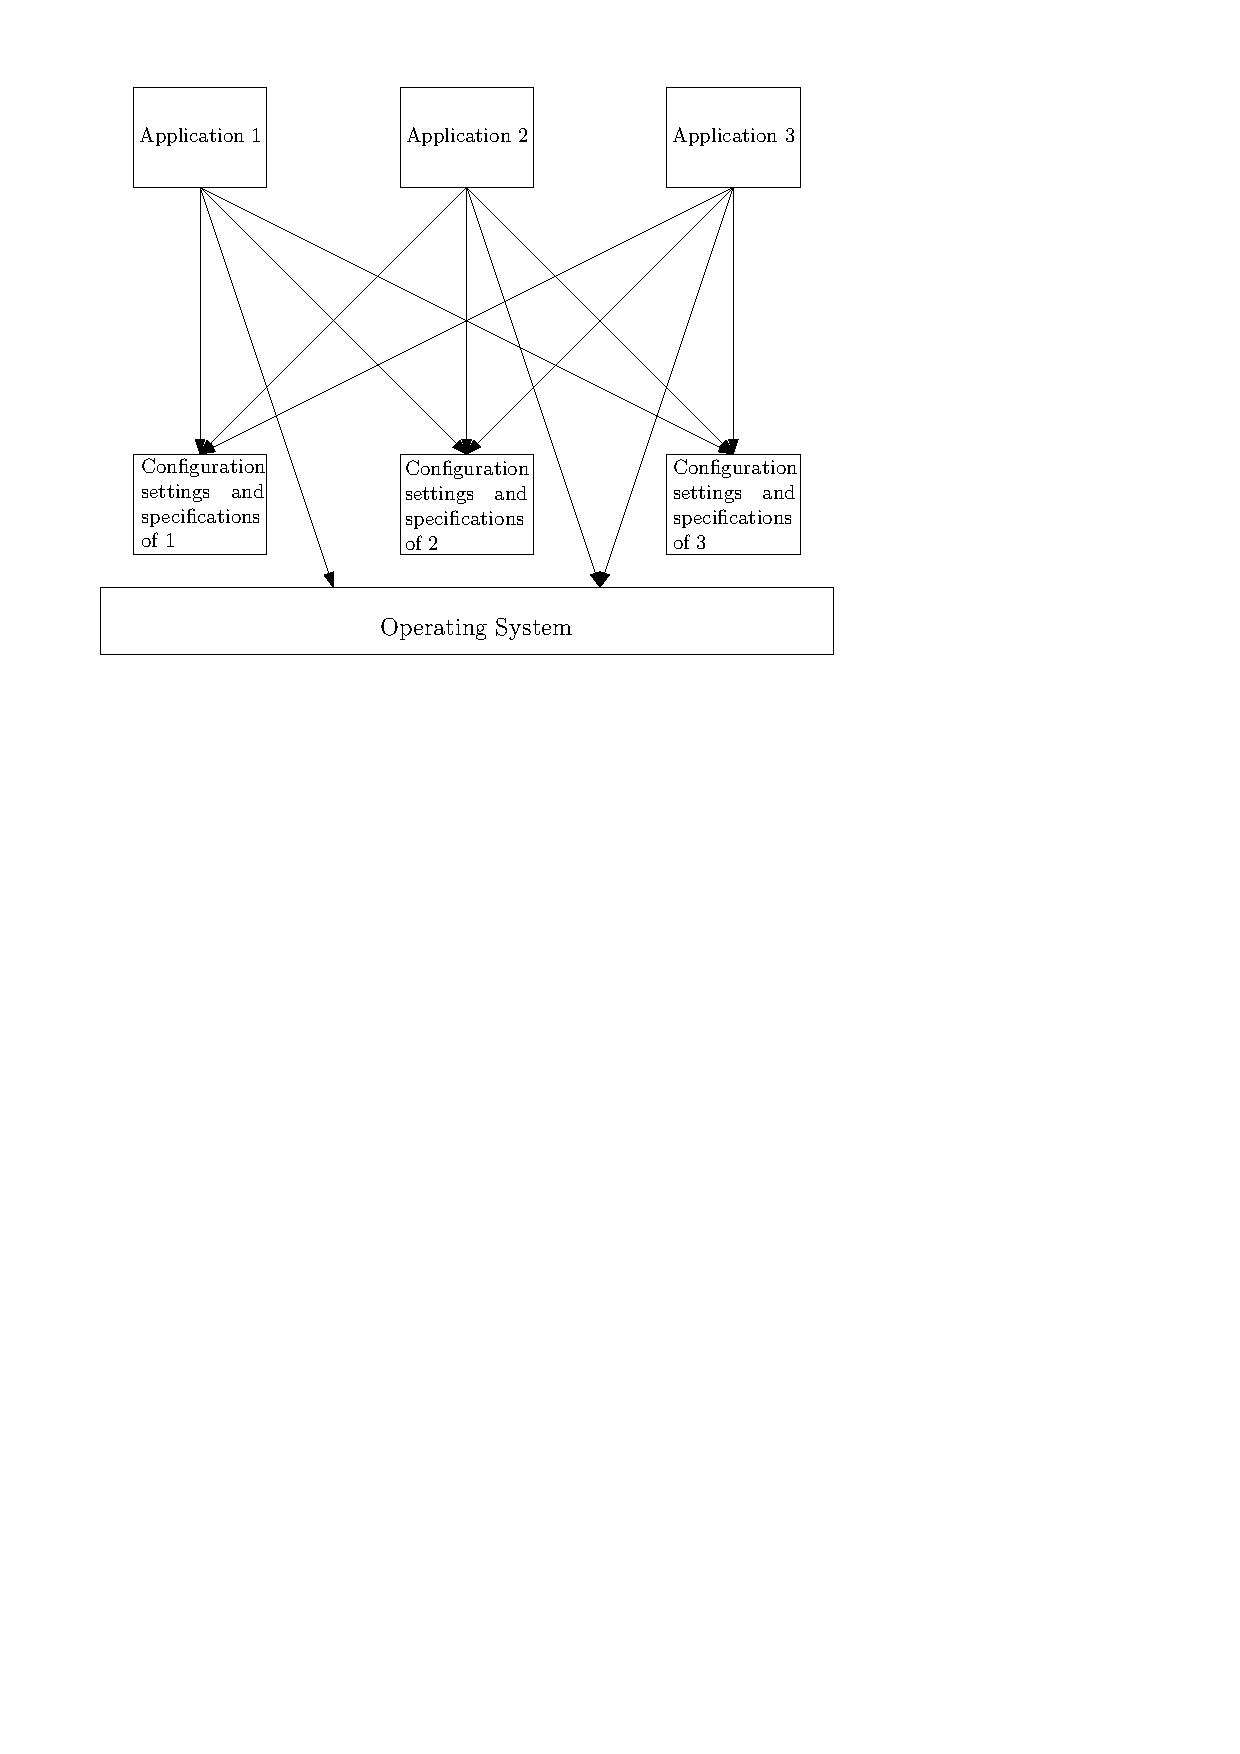
\includegraphics[scale=0.7]{cursituation}
\end{frame}

\begin{frame}
	\frametitle{Wanted Situation}
	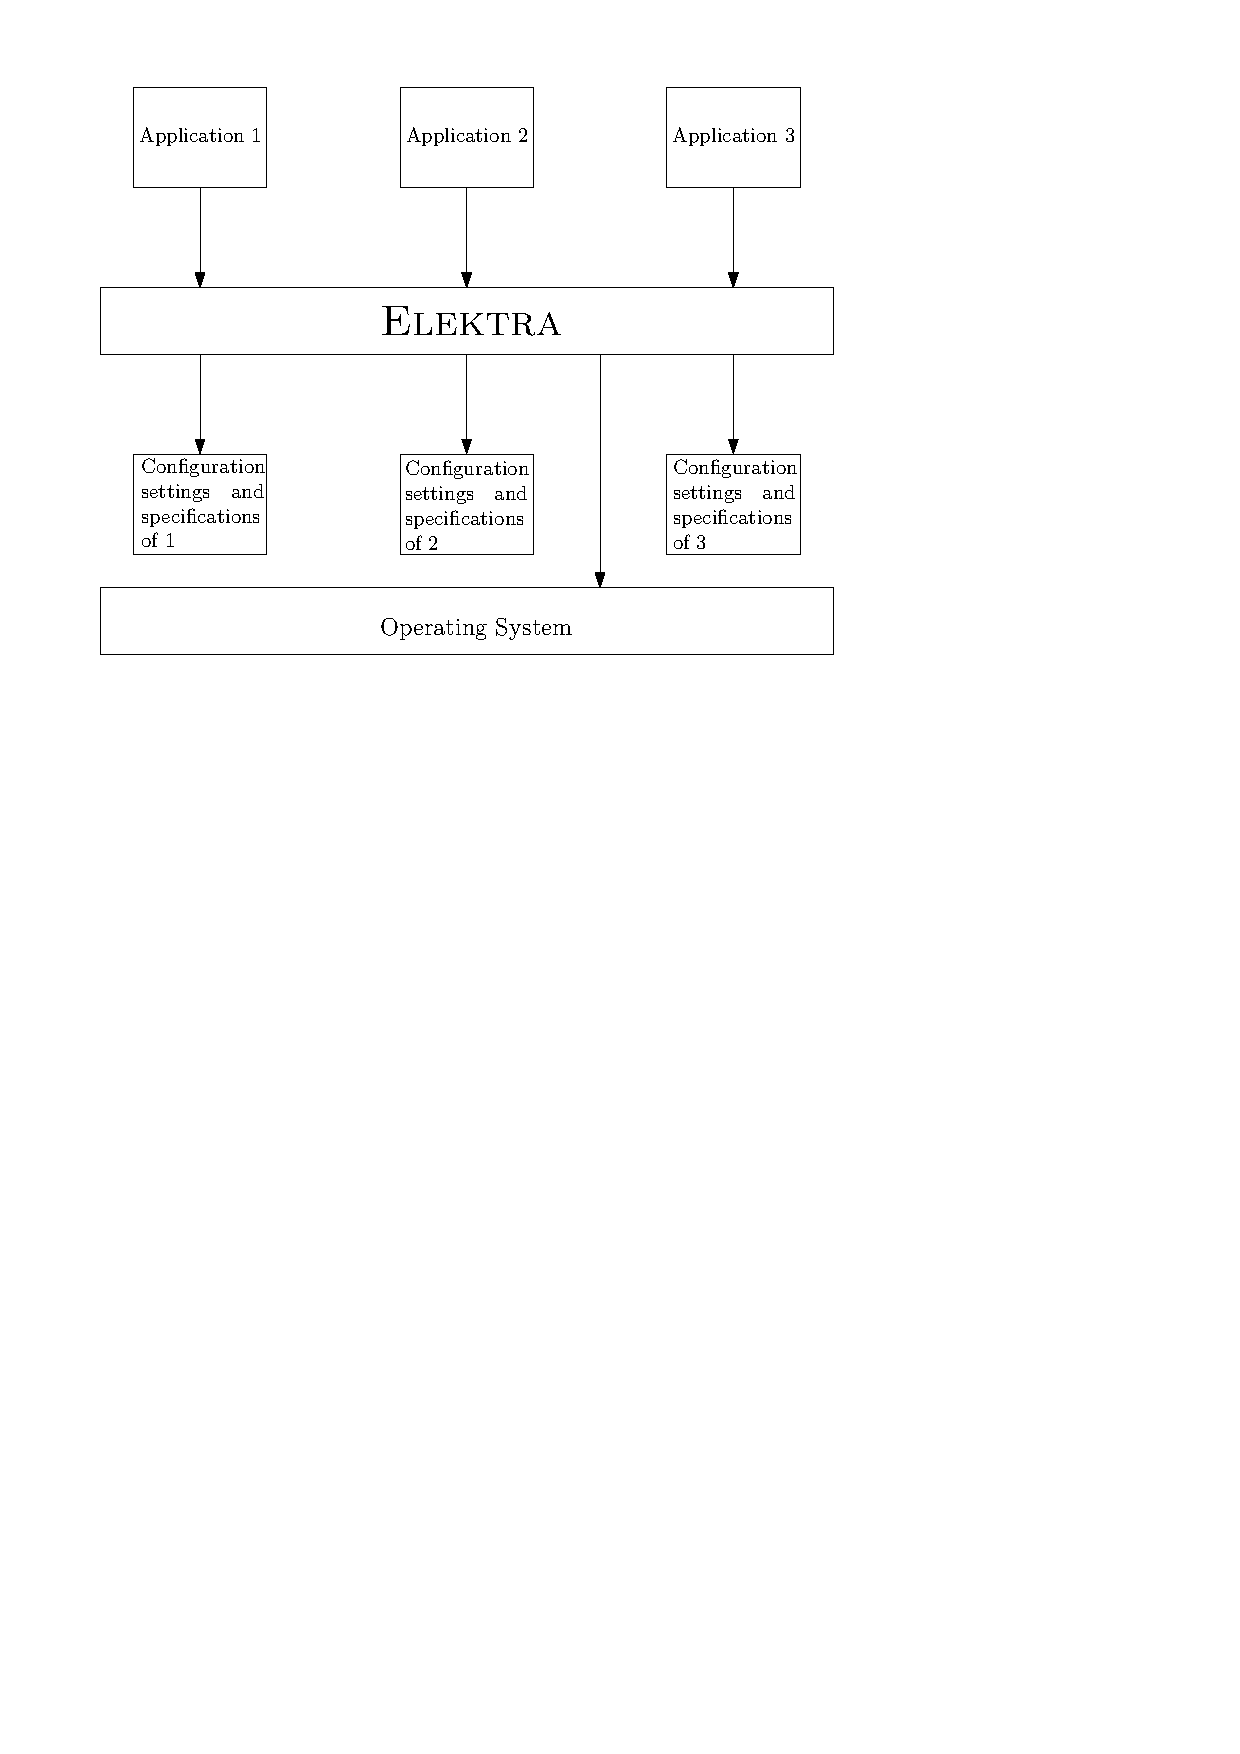
\includegraphics[scale=0.7]{wantsituation}
\end{frame}

\begin{frame}
	\frametitle{Vertical Modularity}
	\begin{alertblock}{Question}
	Explain the content of the figure.
	\end{alertblock}
	\begin{columns}[c]
	\column{7cm}
	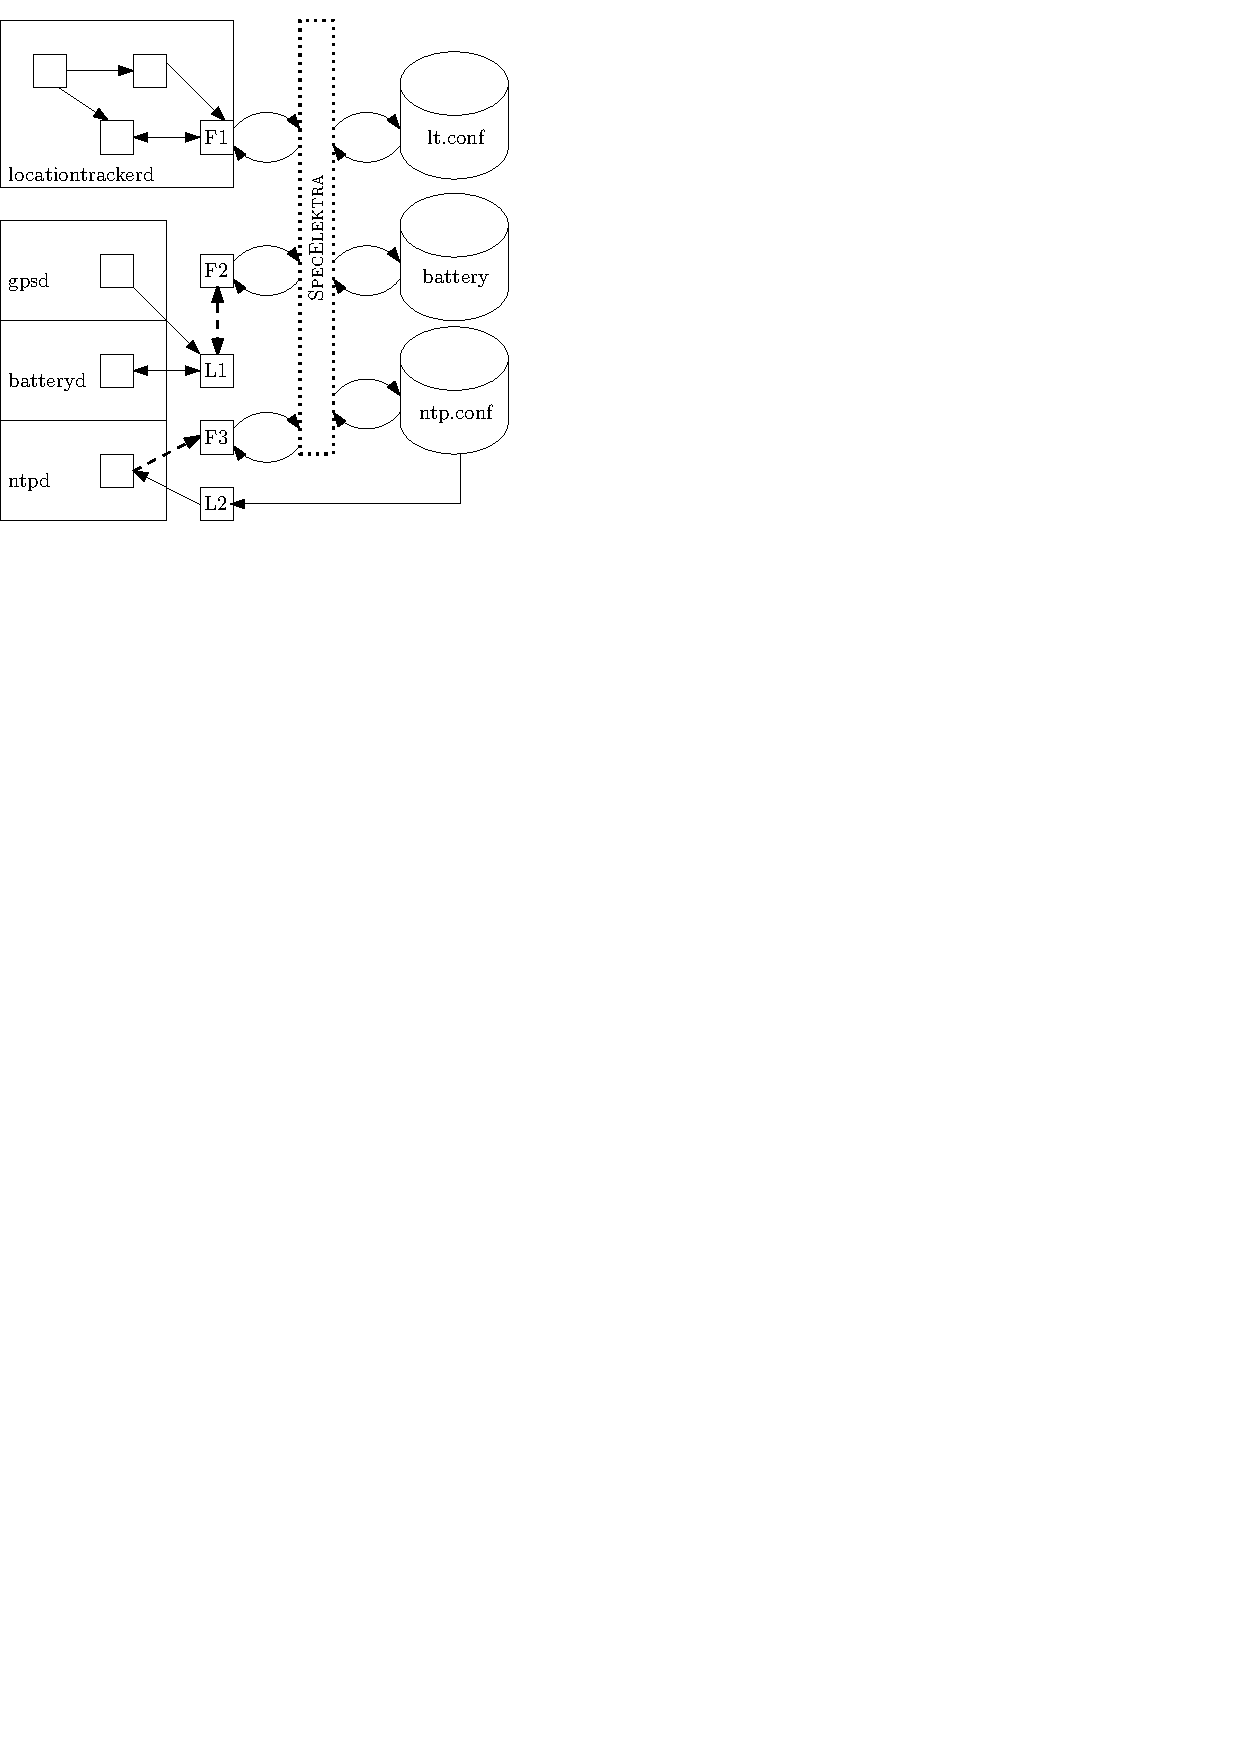
\includegraphics[scale=0.75]{verticalmodularity}
	\column{4cm}<2>
	Needed to keep applications independently.

	Boxes are applications, cylinders are configuration files, F? are frontends or frontend adapters, L? are configuration libraries~\cite{raab2016improving}.
	\end{columns}
\end{frame}

\begin{frame}
	\frametitle{Metalevels (Recapitulation)}
	\begin{alertblock}{Question}
	Describe the three Metalevels in Elektra.
	\end{alertblock}

	\pause
	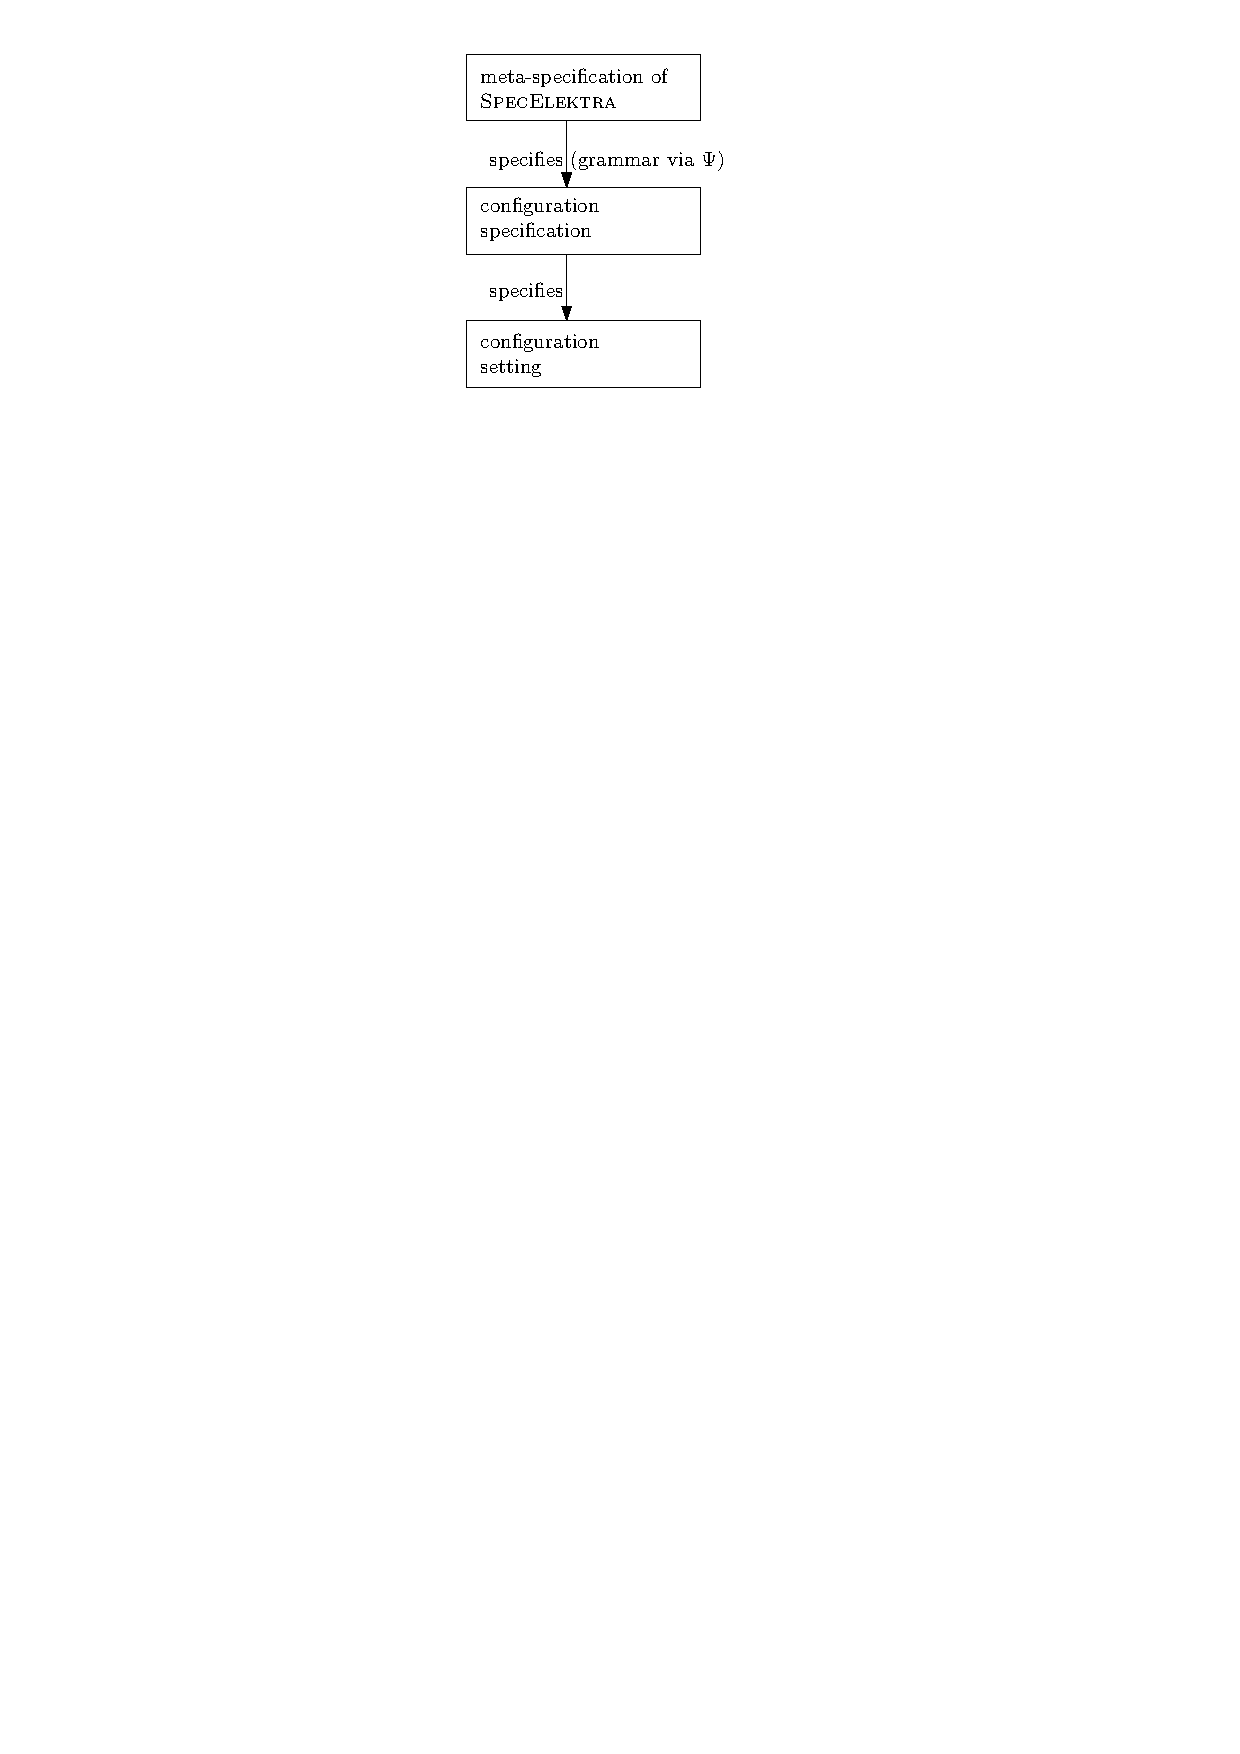
\includegraphics{metalevels}
\end{frame}

\begin{frame}
	\frametitle{Introspection (Recapitulation)}
	\begin{task}
	What is internal and external specification?
	What is introspection?
	\end{task}

	\pause
	\vspace{1em}

	\begin{itemize}
	\item \textit{internal}: within applications' source code
	\item \textit{introspection}: unified get/set access to (meta*)-key/values
	\item access via applications, CLI, GUI, web-UI, ...
	\item access via any programming language (similar to file systems)
	\item GUI, web-UI can semantically interpret metadata
	\item assemble modular parts (validation, logging, \dots)
	\item needed as communication between producers and consumers
	\item essential for \intro[no-futz computing]{no-futz computing}~\citet{holland2001nofutz}
	\end{itemize}
\end{frame}

\begin{frame}
	\frametitle{Introspection vs.\ Code Generation (Recapitulation)}

	\begin{task}
	Advantages/Disadvantages of key database (vs.\ code generation)?
	\end{task}

	\pause

	\setbeamersize{description width=1cm}
	\begin{description}
	\item[$+$] specification can be updated live on the system without recompilation
	\item[$+$] tooling has generic access to all specifications
 	\item[$+$] new features the key database (e.g., better validation) are immediately available consistently
	\item[$-$] less techniques for performance improvements
	\item[$-$] contextual values cannot be used if context differs within same thread
	\end{description}

	\begin{alertblock}{Implication}
	We generally prefer introspection, except for a very thin configuration access API.
	\end{alertblock}
\end{frame}

\begin{frame}
	\frametitle{Definition Configuration Management (Recapitulation)}

	\begin{task}
	What is Configuration Management?
	\end{task}

	\pause

	\begin{itemize}
	\item is a discipline in which configuration (in the broader sense) is administered.
	\item makes sure computers are assembled from desired parts and the correct applications are installed.
	\item has means to describe the desired configuration of the whole managed system.
	\item ensures that the execution environment of installed applications is as required.
	\end{itemize}
\end{frame}

\begin{frame}
	\frametitle{Possible Benefits of CM (Recapitulation)}

	\begin{task}
	What are the goals of Configuration Management?
	\end{task}

	\pause

	\begin{itemize} %[<+-| alert@+>]
	\item The same goals scripts have: \\
		Documentation, Customization, Reproducability
	\item Declarative description of the system \\
		Single Source of Truth 
		(Infrastructure as Code~\cite{waldemar2013testing})
	\item Less configuration drift
	\item Error handling
	\item Pull vs.\ Push
	\item Reusability
	%\item (Resource) Abstractions
	\end{itemize}
\end{frame}

\begin{frame}
	\frametitle{Early detection (Recapitulation)}
	\begin{task}
	When do we want to detect misconfiguration?
	\end{task}

	\pause

	Phases when we can detect misconfigurations:
	\begin{itemize} %[<+-| alert@+>]
	\item Compilation stage in configuration management tool
	\item Writing configuration settings on nodes
	\item Starting applications (load-time)
	\item When configuration setting is actually used (run-time)
	\end{itemize}

	\pause[\thebeamerpauses]

	\begin{alertblock}{Problem}
	Earlier versus more context.
	\end{alertblock}
\end{frame}


\begin{frame}
	\frametitle{Configuration Specification (Recapitulation)}

	\begin{task}
	How can we combine configuration specifications and configuration management?
	\end{task}

	\pause

	\begin{itemize} %[<+-| alert@+>]
	\item configuration settings are simply an instantiation of the configuration specifications.
		Code describing the instantiation is \textbf{CM code}.
	\item configuration design is explicit (like transformations and default values) and can help while writing CM code.
	\item CM code can even be generated from the specification.
	\item access specifications make access trivial via uniform interface.
	\item visibility and similar techniques may help dealing with complexity.
	\end{itemize}
\end{frame}

\begin{frame}
	\frametitle{Properties (Recapitulation)}

	\begin{task}
	What is idempotent, self-describing, round-tripping configuration?
	\end{task}

	\pause


	\begin{description}
	\item[Idempotent]
	yield the same configuration with any number of applications from CM code ($n\ge1$)~\cite{waldemar2013testing}:
	\[
		f(f(x))=f(x)
	\]
	needed to guarantee repeatability

	\item[Self-describing]
	means that from the configuration file alone we are able to derive the correct data structure~\cite{wadler2003xml}.

	\item[Round-tripping]
	means that if a data structure is serialized and then parsed again, we end up with an identical data structure~\cite{wadler2003xml}.
	\end{description}

	The data structure could be a KeySet.
\end{frame}

\begin{frame}
	\frametitle{Popular CMs today (Recapitulation)}

	\begin{itemize} %[<+-| alert@+>]
	\item CFengine (1993)
	\item LCFG (1994)
	\item Quattor (2005)
	\item Puppet (2005)
	\item Chef (2009)
	\item Salt (2011)
	\item Ansible (2012)
	\item Mgmt (2016)
	\item OpsMops (2019)
	\end{itemize}
\end{frame}

\begin{frame}
	\frametitle{Elektra (Recapitulation)}

	\begin{task}
	What is Elektra?
	\end{task}

	\pause

	\begin{itemize}
	\item is not only a key database but a specification language to describe a key database
	\item plugins implement the specification (could be distributed but focus is configuration files)
	\item is library based (no single point of failure, no distributed coordination needed)
	\item supports transactions (persisting whole KeySets at once)
	\item supports integration of existing configuration settings
	\end{itemize}
\end{frame}


\begin{frame}
	\frametitle{Error Messages (Recapitulation)}

	\begin{task}
	What needs to be considered when designing error messages?
	\end{task}

	\pause

	\begin{itemize} %[<+-| alert@+>]
	\item error messages are often the sole data source for admins
	\item configuration design first: avoid errors if possible
	\item error messages should not leak internals~\cite{brown1983error}
	\item ``edit here mentality'': do not point to correct statements~\cite{marceau2011mind}
	\item Precisely locate the cause (and do not report aftereffects)
	\item Personification~\cite{lee2011personifying}
	\item give context: providing enough information vs.\ not overwhelming the user~\cite{wrenn2017error}

	%mixture from other slides:
	\item pin-point key (which also pin-points to the specification)
	\item let specifications, e.g.\ from validation, override messages
	\end{itemize}
\end{frame}




\subsection{}

\begin{frame}
	\frametitle{CM Languages (Partly Recapitulation)}

	\begin{itemize}[<+-| alert@+>]
	\item What is the relationship to software configuration management (Proteus/PCL)?
	\item[] Build systems may provide configuration management features.
	\item How is it possible to provide referential transparency both for the configuration specification language and for the system itself (NIX, GNU Guix)?
	\item[] By functional languages and file system (layouts).
	\item Which notations for CM exist?
	\item[] Text,  Graphical (UML), Semi-structured, Key-value, Structured
	\end{itemize}
\end{frame}


\begin{frame}
	\frametitle{Apply to CM (Recapitulation)}

	What can we learn from system administration research?

	\setbeamersize{description width=1cm}
	\begin{description}[<+-| alert@+>]
	\item[$+$] intensive review process catches errors
	\item[$-$] collaboration ineffective
	\item[$-$] context/situational awareness is essential
	\item[$+$] precise editing of configuration files works well
	\item[$+$] self-written tools are very efficient
	\item[$-$] global optimizations difficult
	\end{description}

	\pause[\thebeamerpauses]  %  show after \begin{itemize}[<+->]

	\begin{alertblock}{Idea}
	Replicate parts that work well, automate error-prone parts.
	\end{alertblock}
\end{frame}

\begin{frame}
	\frametitle{Apply to Elektra (Recapitulation)}

	Elektra's goals are that it should:

	\begin{itemize}[<+-| alert@+>]
	\item be easy to develop new high-level tools
	\item support manual workflows and scripts
	\item support precise editing:\\ only change the configuration value as specified
	\item provide a language for both devs and admins
	\end{itemize}

	\pause[\thebeamerpauses]  %  show after \begin{itemize}[<+->]

	Admins/devs still need to:

	\begin{itemize}[<+-| alert@+>]
	\item reduce the configuration space
	\item intensively review and improve the specifications
	\item test (and debug) configuration settings
	\end{itemize}
\end{frame}

\begin{frame}
	\frametitle{Precise Editing (Recapitulation)}

	Partial modifications (precise editing) is natural for humans. \\
	It ensures preservations of (potentially security-relevant!) defaults. \\
	In CM following methods are used:

	\begin{itemize}[<+-| alert@+>]
	\item embed shell commands to do the work
	\item replace full content of configuration files
	\item replace full content of configuration files with templates
	\item line based manipulation (e.g., file\_line): match line and replace it
	\item Augeas/XML: match a key with XPath and replace it
	\item Elektra: set the value of a key
	\end{itemize}
\end{frame}




%%%%%%%%%%%%%%%%%%%%%%%%%%%%%%%%%%%%%%%%%% 
\section{Configuration Management}

\begin{frame}[fragile]
	Key/value access in Chef:

	\begin{code}[morekeywords={kdbset,do,action,value,end},gobble=4]
	kdbset 'system/sw/samba/global/workgroup' do
		value 'MY_WORKGROUP'
		action :create
	end
	\end{code}
\end{frame}

\begin{frame}[fragile]
	Key/value access in Ansible:

	\begin{code}[morekeywords={name,connection,key,value,elektra,mountpoint,file,plugins,hosts,tasks},gobble=4]
	- name: setup samba
	  connection: local
	  hosts: localhost
	  tasks:
	  - name: set workgroup
	    elektra:
	      mountpoint: system/sw/samba
	      file: /etc/samba/smb.conf
	      plugins: ini
	    elektra:
	      key: 'system/sw/samba/global/workgroup'
	      value: 'MY_WORKGROUP'
	\end{code}
\end{frame}

\begin{frame}[fragile]
	Key/value access in puppet-libelektra:

	\begin{code}[morekeywords={kdbkey,kdbmount,ensure,value},gobble=4]
	kdbmount {'system/sw/samba':
		ensure => 'present',
		file => '/etc/samba/smb.conf',
		plugins => 'ini'
	}
	kdbkey {'system/sw/samba/global/workgroup':
		ensure => 'present',
		value => 'MY_WORKGROUP'
	}
	kdbkey {'system/sw/samba/global/log level':
		ensure => 'absent'
	}
	\end{code}

	Uniqueness of keys is essential.
	Ideally, applications already mount their configuration at installation.
\end{frame}


\begin{frame}[fragile]
	Key/value specifications in puppet-libelektra:

	\begin{code}[morekeywords={kdbkey,ensure,value},gobble=4]
	kdbkey {'system/sw/samba/global/log level':
		ensure => 'present',
		value => 'MY_WORKGROUP',
		check => {
			'type' => 'short',
			'range' => '0-10',
			'default' => '1',
			'description' => 'Sets the amount of log/
				debug messages that are sent to the
				log file. 0 is none, 3 is consider-
				able.'
	}
	\end{code}

	Ideally, applications already specify their settings.
\end{frame}

\begin{frame}
	\frametitle{Key/Values Revisited}

	Decide about \textbf{changeability} per key:

	\begin{itemize}[<+-| alert@+>]
	\item Who is responsible (end user, packages, admin manual or CM).
	\item In which namespaces apps search the key (cascading lookup).
	\item Who can see it (visibility).
	\item Who can edit it (admin, end user, both).
	\item Which configuration values are allowed (validation).
	\end{itemize}

	\pause[\thebeamerpauses]  %  show after \begin{itemize}[<+->]

	\begin{alertblock}{Changeability}
	Ownership of every key must be very clear and documented.
	\end{alertblock}
\end{frame}

\begin{frame}[fragile]
	Key/value specifications in puppet-libelektra:

	\begin{code}[morekeywords={kdbkey,ensure,value},gobble=4]
	kdbkey {'spec/xfce/pointers/Mouse/RightHanded':
		ensure => 'present',
		check => {
			'namespaces/#0' => 'user',
			'namespaces/#1' => 'system',
			'visibility' => 'important',
			'default' => 'false',
			'check/type' => 'boolean'
	}
	\end{code}

	Ideally, applications already specify their settings.
\end{frame}

\begin{frame}
	\frametitle{Layers of Abstractions}

	Recursively define useful abstractions (meta-levels):

	\begin{itemize}[<+-| alert@+>]
	\item Bits in (configuration) files and memory
	\item Key/value view of configuration settings
	\item Goals/specifications of settings per node and instantiations of modules
	\vspace{1em}
	\item CM code to instantiate settings in the whole network
	\item Global optimization: allocation of nodes and decision regarding topology in the whole network
	\item Global goals/specifications of the whole network
	\end{itemize}
\end{frame}

\begin{assignment}
	\begin{task}
	Break.
	\end{task}
\end{assignment}

\begin{frame}
	\frametitle{Design Rules~\cite{burgess2006modeling}}

	\begin{itemize}[<+-| alert@+>]
	\item Factor processes into containers to avoid overlaps in settings.
	\item Maintain clear separation of ownership (for every key).
	\item Specify replicated settings in a single source (use links and derivations).
	\item Document all remaining overlaps (in the specification).
	\item The manageability of settings is reduced by the number of possible configuration values.
	\item Do not separate configuration management and monitoring. % TODO: rethink
	\end{itemize}
\end{frame}


\begin{frame}
	\frametitle{Open Topics}

	\begin{itemize}[<+-| alert@+>]
	\item global optimizations/self-healing
	\item configuration integration
	\item safe migrations of settings and data
	\item collaboration
	\item management (including knowledge)
	\item centralized vs.\ distributed
	\end{itemize}
\end{frame}


\begin{frame}
	\frametitle{Conclusion}

	\begin{itemize}[<+-| alert@+>]
	\item have unique identifier for your configurations settings (get/set key/values)
	\item be aware of the specifications, solving CM is solving constraints
	\item do not design around tools but design tools around you
	\item be brave and remove all configuration settings you can
	\item use all help you can get: e.g.\ build tools, preseeding, installer automation, virtualization, package managers, distributions
	\item complexity in CM vs.\ complexity in applications' specification
	\item modularity is essential for validation and legacy support
	\item artifact generation improves consistency and type safety
	\end{itemize}
\end{frame}

\begin{assignment}
	\begin{task}
	Feedback.
	\end{task}
\end{assignment}




%%%%%%%%%%%%%%%%%%%%%%%%%%%%%%%%%%%%%%%%%% 
\nocite{raab2017introducing}

\appendix

\begin{frame}[allowframebreaks]
	\bibliographystyle{plainnat}
	\bibliography{../shared/elektra.bib}
\end{frame}

\end{document}

